% Adapted to the Springer Nature (sn-jnl) template.
% Version 3.1 December 2024

\documentclass[pdflatex,sn-mathphys-num]{sn-jnl}% Math and Physical Sciences Numbered Reference Style

%%%% Standard Packages
\usepackage{graphicx}%
\usepackage{multirow}%
\usepackage{amsmath,amssymb,amsfonts}%
\usepackage{amsthm}%
\usepackage{mathrsfs}%
\usepackage{xcolor}%
\usepackage{textcomp}%
\usepackage{booktabs}%
%%%%

\raggedbottom

\begin{document}

\title[Resource-state modulation of prefrontal value processing]{Resource-State Modulation of Prefrontal Value Processing during Earning--Spending Decision Making}

%%=============================================================%%
%% GivenName	-> \fnm{Joergen W.}
%% FamilyName	-> \sur{Ploeg}
%% \author*[1,2]{\fnm{Joergen W.} \sur{Ploeg}}\email{iauthor@gmail.com}
%%=============================================================%%

\author[1,2]{\fnm{Hualei} \sur{Wang}}

\author[1,2]{\fnm{Hangyu} \sur{Si}}

\author*[1]{\fnm{Tianming} \sur{Yang}}\email{tyang@ion.ac.cn}

\affil*[1]{\orgdiv{Center for Excellence in Brain Science and Intelligence Technology (Institute of Neuroscience)}, \orgname{Chinese Academy of Sciences}, \orgaddress{\city{Shanghai}, \postcode{200031}, \country{China}}}

\affil[2]{\orgname{University of Chinese Academy of Sciences}, \orgaddress{\city{Beijing}, \postcode{100049}, \country{China}}}

\abstract{The trade-off between earning and spending is fundamental to economic life, yet its neural basis remains poorly understood. To address this question, three macaque monkeys were trained on a novel earning--spending task in which they chose between earning virtual tokens and spending accumulated tokens for immediate juice rewards. Tokens carried over across trials, enabling animals to accumulate wealth over time and defer spending until favorable opportunities arose. Spending preferences increased systematically with accumulated wealth, consistent with the principle of diminishing marginal utility. Electrophysiological recordings across three prefrontal subregions revealed differential encoding patterns. The anterior cingulate cortex (ACC) most robustly encoded and dynamically updated current wealth following each choice outcome. The orbitofrontal cortex (OFC) encoded wealth alongside values and good-based (earning vs.\ spending) choice signals. The dorsolateral prefrontal cortex (DLPFC) predominantly encoded choice in the action domain (left vs.\ right), with comparatively weaker wealth and value signals. These results reveal a coordinated division of labor within the prefrontal cortex that supports wealth-dependent economic decision-making.}

\keywords{Wealth, Token, Earning--spending, Orbitofrontal cortex, Anterior cingulate cortex, Value-based decision making, Diminishing marginal utility}

\maketitle

\section{Introduction}\label{sec1}

Whether to work late for an extra paycheck or leave early to enjoy the evening---decisions between earning and spending are among the most fundamental in economic life, and are profoundly shaped by current wealth. The relationship between wealth and economic decision has been formalized by expected utility theory, in which a concave utility function captures the diminishing marginal value of resources \cite{bernoulli1954exposition, von1947theory}. A central prediction follows: as wealth accumulates, risk aversion decreases and behavior converges toward the rational ideal. Human behavioral data support this account across multiple domains and ages---from labor supply and prosocial behavior in adults \cite{cesarini2017effect, vanags2025greater} to risk sensitivity in children as young as four \cite{harvey2022developmental}. This framework extends to non-human primates (NHP), which can acquire tokens as symbolic wealth \cite{sousaUseTokensRewards2001, chenHowBasicAre2006a, addessiAreRootsHuman2020, beran2021non, leca2021acquisition, seo2009behavioral} and whose economic preferences are systematically shaped by accumulated token holdings \cite{yangPrimateAnteriorInsular2022c, ferroAccumulationVirtualTokens2025a}.

Because wealth-dependent decisions are, at their core, value-based choices, they naturally engage the distributed prefrontal value network, in which OFC, DLPFC, and ACC make distinct contributions: OFC encodes the subjective value of available options \cite{padoa-schioppaNeuronsOrbitofrontalCortex2006b, padoa-schioppaOrbitofrontalCortexNeural2017, rudebeckOrbitofrontalCortex2018, ballestaValuesEncodedOrbitofrontal2020a, ballestaOrbitofrontalCortexContributes2022}; DLPFC facilitates choice in the spatial domain and modulates value representation through cognitive control \cite{cai2014contributions, lin2021evidence, hareSelfControlDecisionMakingInvolves2009, mcclureSeparateNeuralSystems2004a, fignerLateralPrefrontalCortex2010a}; ACC integrates value with action costs and drives behavioral switching \cite{haydenNeuronalBasisSequential2011a, amemoriLocalizedMicrostimulationPrimate2012a, caiNeuronalEncodingSubjective2012, kennerleyNeuronsFrontalLobe2009b, prevostSeparateValuationSubsystems2010b, kollingNeuralMechanismsForaging2012a}. Based on this foundational computation, wealth itself is represented as a dynamic reference point that modulates value encoding across OFC, ACC, and vmPFC as token holdings change \cite{yangPrimateAnteriorInsular2022c, juechemsVentromedialPrefrontalCortex2017, nguyenNeuralRepresentationDecisional2025a}. Yet existing token paradigms share two structural limitations: fixed exchange thresholds introduce uncontrolled reference points, and options remain confined to the token gain--loss domain---varying how many tokens are earned or lost---without ever placing earning and spending in direct competition as explicit choice alternatives. No study has examined how accumulated wealth shapes this fundamental trade-off, one of the most elemental decisions in economic life.

Here we trained three rhesus monkeys on a novel earning--spending task in which, on each trial, the animal chose between acquiring an additional token or spending accumulated tokens for immediate juice reward. We analyzed behavior and neural activity within an expected utility framework. Monkeys' tendency to spend increased as token wealth accumulated, providing the first evidence of wealth-dependent earning--spending behavior in NHP. Electrophysiological recordings across three prefrontal subregions revealed a coordinated division of labor, with distinct regions differentially encoding wealth state, wealth-dependent value, and choice. These findings provide a neural account of how accumulated wealth shapes the earn--spend trade-off, illuminating a fundamental yet previously unexplored dimension of economic decision-making.

\section{Results}\label{sec2}

\begin{figure}[htbp]
\centering
\includegraphics[width=\textwidth]{Figure1}
\caption{
\textbf{(A) Task design.} The yellow circle array at the center represents the monkey's ``wallet,'' which remained visible during the inter-trial interval (ITI) to provide a continuous representation of wealth. Each trial began with two geometric shapes representing earning and spending options presented on a computer screen. Monkeys indicated their choice by directing a saccade to a target and maintaining fixation for a required duration. Outcomes were delivered incrementally during fixation as tokens were added to or deducted from the wallet, with juice rewards delivered at the moment of each token deduction. Monkeys could switch between options via saccade.
\textbf{(B) Task conditions.} Twelve experimental conditions were defined by crossing three earning options ($V_\text{Earn}$, earning speed) with four spending options ($V_\text{Spend}$, reward magnitude). Each spending option cost one token and yielded a juice reward of the corresponding magnitude; each earning option yielded one token at the corresponding speed. The red-to-green gradient in the contingency matrix indicates the objective value ratio ($V_\text{Earn}/V_\text{Spend}$), where red and green denote conditions objectively favoring earning and spending, respectively.
\textbf{(C) Behavioral summary.} Each row corresponds to one monkey; the four columns show behavioral choice patterns, subjective weights, psychometric curves, and reaction time distributions, respectively. \textbf{Behavioral choice pattern.} Earning percentage is plotted across 24 token levels for each of the 12 offer conditions. The red--green color gradient encodes the objective value condition; luminance encodes current wealth. Only the first choice in each trial is included. \textbf{Subjective weights.} Non-parametric weights for each shape are plotted as a function of token count, illustrating how current wealth reshapes the perceived value of each offer. \textbf{Psychometric curves.} Earning percentage is plotted against the estimated value difference ($\Delta V = V_\text{Earn} - V_\text{Spend}$). Each point represents the earning percentage for a specific offer--wealth combination, with point color following the same offer-condition convention as column 1; point size is proportional to the number of observations. The curve is a logistic function fitted to the data. \textbf{Reaction time distributions.} Trials were divided into ``easy'' ($|\Delta V|$ above median) and ``hard'' ($|\Delta V|$ below median) groups. Histograms show reaction-time (RT) distributions of the first choice for each group; choices with smaller value differences elicited longer deliberation (Wilcoxon rank-sum test: $p = 1.3 \times 10^{-191}$ for monkey W, $p < 10^{-300}$ for monkey U, and $p = 4.8 \times 10^{-223}$ for monkey T).
}
\label{fig:1}
\end{figure}

\subsection{Wealth-dependent earning--spending trade-off}

Three rhesus macaques were trained on a novel earning--spending task (Fig.~\ref{fig:1}A) that required them to choose between earning virtual tokens and spending accumulated tokens for juice rewards. Each trial presented two options characterized by distinct earning speeds ($V_\text{Earn}$) and reward magnitudes ($V_\text{Spend}$) (Fig.~\ref{fig:1}B). Critically, tokens earned in any given trial carried over to subsequent trials until spent, incentivizing a strategy of accumulating wealth during high-earning periods and deferring expenditure until high-spending opportunities arose.

Analysis of the initial choice in each trial revealed that monkeys optimized their behavior according to both the current offer conditions and their accumulated wealth (Fig.~\ref{fig:1}C, column 1). While higher $V_\text{Earn}$ and lower $V_\text{Spend}$ increased the probability of choosing to earn, current wealth also biased this trade-off. Non-parametric estimation of subjective weights for the seven option shapes across all 24 wealth levels revealed that these weights varied with wealth in an option-dependent manner: weights assigned to earning options decreased as wealth accumulated, whereas those assigned to spending options increased (Fig.~\ref{fig:1}C, column 2). This systematic shift is consistent with the principle of diminishing marginal utility, suggesting that wealth reshapes the perceived value of economic options.

To characterize the computational mechanism underlying these choices, we developed a parametric model grounded in marginal utility theory (see Methods). The model captured individual choice patterns, as reflected by the close correspondence between psychometric curves and the estimated value difference $\Delta V = V_E - V_S$ (Fig.~\ref{fig:1}C, column 3), where $V_E$ and $V_S$ were subjective values estimated by the model. Moreover, $|\Delta V|$ predicted decision effort: trials with smaller value differences elicited significantly longer reaction times, indicating increased deliberation during difficult trade-offs (Fig.~\ref{fig:1}C, column 4). Together, these results demonstrate that macaques assign wealth-dependent subjective values to economic options and make decisions in accordance with those values.

\begin{figure}[htbp]
\centering
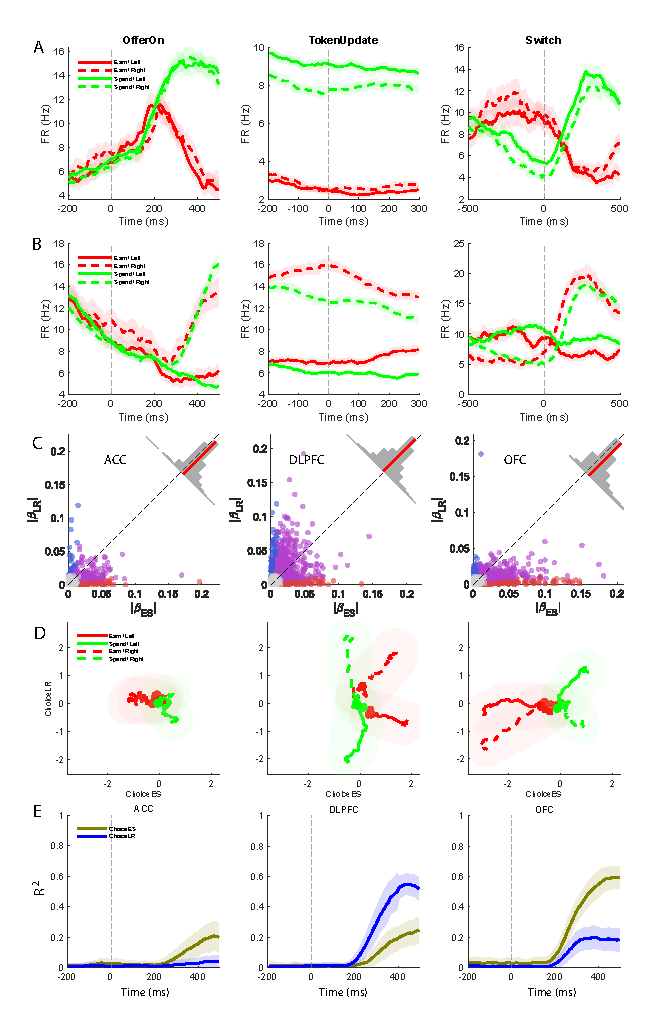
\includegraphics[width=\textwidth]{Figure2}
\caption{\textbf{Neural Dissociation of Good-based and Action-based Choice.} \textbf{(A--B) Representative example units.} Firing rates (mean $\pm$ SEM) of a representative OFC neuron selective for the earning/spending domain (A) and a DLPFC neuron selective for the left/right domain (B), aligned to offer onset (left), token update (middle), and switch (right). Responses are grouped by Earning (red)/Spending (green) $\times$ Left (solid)/Right (dashed). \textbf{(C) Summary of single-unit selectivity.} Each dot represents one neuron, plotted by its absolute regression coefficient for the earning/spending (ES, $x$-axis) and left/right (LR, $y$-axis) domains. Colors indicate significance ($p < 0.05$): red (ES only), blue (LR only), purple (both), gray (neither). The inset histogram, oriented along the anti-diagonal, shows the population distribution of relative LR-versus-ES selectivity ($\propto (|\beta_{LR}| - |\beta_{ES}|)$); a shift toward the top left indicates LR dominance. The ACC and OFC are predominantly ES-selective (binomial test: $p = 1.09 \times 10^{-31}$ and $p = 2.67 \times 10^{-48}$, respectively), while the DLPFC is predominantly LR-selective ($p = 3.97 \times 10^{-4}$). \textbf{(D) Neural trajectories in ES--LR space.} Population dynamics projected onto the ES and LR axes derived via TDR, for ACC (left), DLPFC (middle), and OFC (right). Red/green lines indicate earning/spending choices; solid/dashed lines indicate left/right choices. Shaded regions show the spatial dispersion ($\pm$SD) across trial resamples. \textbf{(E) Temporal encoding dynamics.} Encoding strength ($R^2$, squared Pearson correlation between population projection and choice label) on the ES (yellow) and LR (blue) axes as a function of time. Shaded regions show $\pm$SD across 100 bootstrap iterations.}
\label{fig:2}
\end{figure}

\subsection{Good-based vs.\ Action-based Choice Representation}
Choices in this task are defined simultaneously in the good-based domain (earning vs.\ spending) and in the action-based domain (left vs.\ right). Figure~\ref{fig:2}A and B show representative neurons illustrating this dissociation at the single-unit level: the example OFC neuron (Fig.~\ref{fig:2}A) modulates its firing rate with the earning/spending identity of the chosen option, whereas the example DLPFC neuron (Fig.~\ref{fig:2}B) tracks the left/right action of the response. Across the recorded population, the scatter of regression coefficients (Fig.~\ref{fig:2}C) confirms that this specialization is systematic: neurons in the OFC and ACC are biased toward the ES domain, while neurons in the DLPFC are biased toward the LR domain, with many individual neurons showing mixed selectivity for both. To characterize how these signals are organized at the level of the full population, we applied Targeted Dimensionality Reduction (TDR; \citep{mante2013context}), which demixed task variables at the population level by constructing orthogonal population axes. The resulting neural trajectories and encoding dynamics (Fig.~\ref{fig:2}D--E) reveal differential representation across prefrontal subregions: the OFC and ACC preferentially represent good-based information, while the DLPFC specializes in action-based information.

\begin{figure}[htbp]
\centering
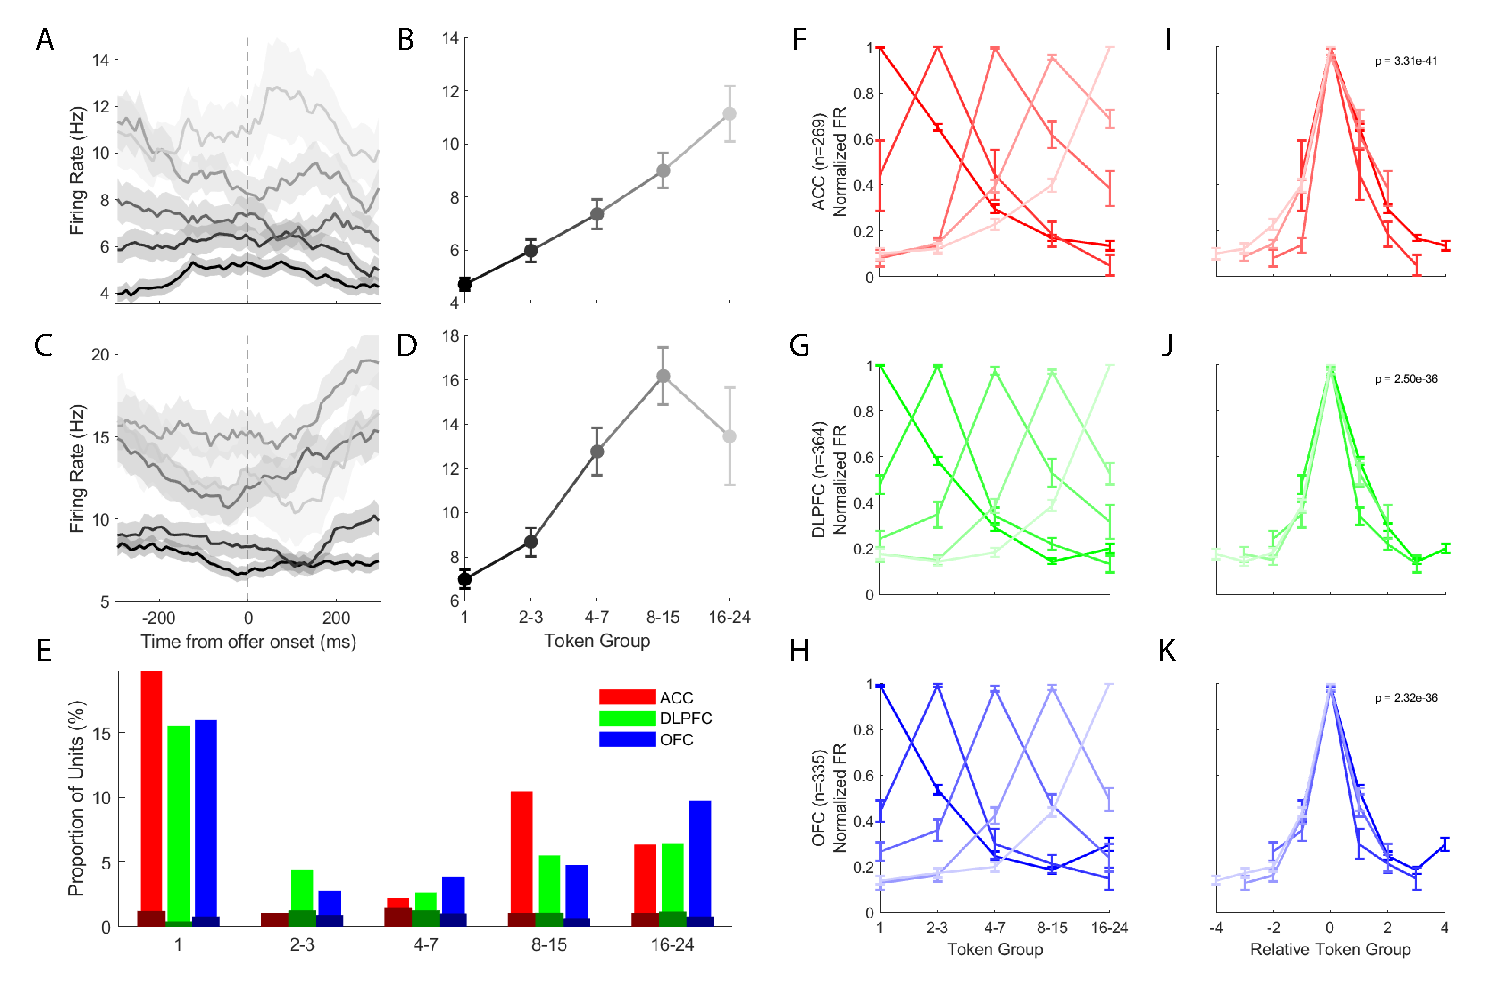
\includegraphics[width=0.7\textwidth]{Figure3_1}
\caption{\textbf{Wealth tuning curve.} \textbf{(A--D) Representative units with wealth encoding.} Firing rates (mean $\pm$ SEM) of two example neurons aligned to offer onset (A and C) and corresponding tuning curves (B and D). Trials are grouped into five wealth levels ([1], [2--3], [4--7], [8--15], [16--24]; dark-to-light color gradient indicates increasing wealth). The unit shown in (A) and (B) exhibits monotonic tuning, with firing rate increasing toward the ``rich'' wealth extreme. The unit shown in (C) and (D) exhibits categorical tuning peaking at the intermediate level [8--15], revealing a non-monotonic profile. \textbf{(E) Preferred wealth level distribution.} Proportion of wealth-selective neurons in each brain area preferring each wealth level. Gray bars are shuffle controls. \textbf{(F--K) Population tuning curves.} Normalized and averaged tuning curves for neurons grouped by preferred wealth level in ACC (F, I), DLPFC (G, J), and OFC (H, K). Panels I--K show the same curves re-centered relative to each group's preferred wealth level. Wilcoxon rank-sum test $p$-values comparing normalized firing rates at relative positions $\pm1$ versus $\pm2$ from the peak are annotated in each panel.}
\label{fig:3_1}
\end{figure}

\subsection{Wealth Selectivity}
Neuronal encoding of wealth followed two distinct patterns: monotonic and non-monotonic (categorical). Monotonic neurons represented wealth along a continuous gradient, preferring either the ``rich'' or ``poor'' extreme (Fig.~\ref{fig:3_1}A, B), whereas categorical neurons exhibited discrete tuning to specific wealth levels (Fig.~\ref{fig:3_1}C, D). Wealth-selective neurons were distributed across all three prefrontal regions, and the proportion of neurons preferring each wealth level formed a prominent U-shaped distribution, with neurons preferring the boundary wealth states ([1] and [16--24]) being most prevalent (Fig.~\ref{fig:3_1}E). Grouping neurons by their preferred wealth level and averaging their normalized tuning curves revealed consistent tuning profiles across all groups (Fig.~\ref{fig:3_1}F--H). When re-centered relative to each group's preferred wealth level, the population tuning curves exhibited a systematic, graded decline with increasing distance from the peak (Fig.~\ref{fig:3_1}I--K). A Wilcoxon rank-sum test confirmed that normalized firing rates at relative positions $\pm1$ were significantly higher than those at $\pm2$ ($p = 3.31 \times 10^{-41}$, $2.50 \times 10^{-36}$, and $2.32 \times 10^{-36}$ for ACC, DLPFC, and OFC, respectively), indicating that the tuning curves reflect genuine graded encoding rather than an isolated peak driven by noise; this conclusion is further supported by the shuffle controls presented in Fig.~S6. Collectively, by spanning the full range of possible wealth states, these heterogeneously tuned neurons enable the prefrontal network to maintain a continuous and comprehensive representation of the subject's current economic status.

\begin{figure}[htbp]
\centering
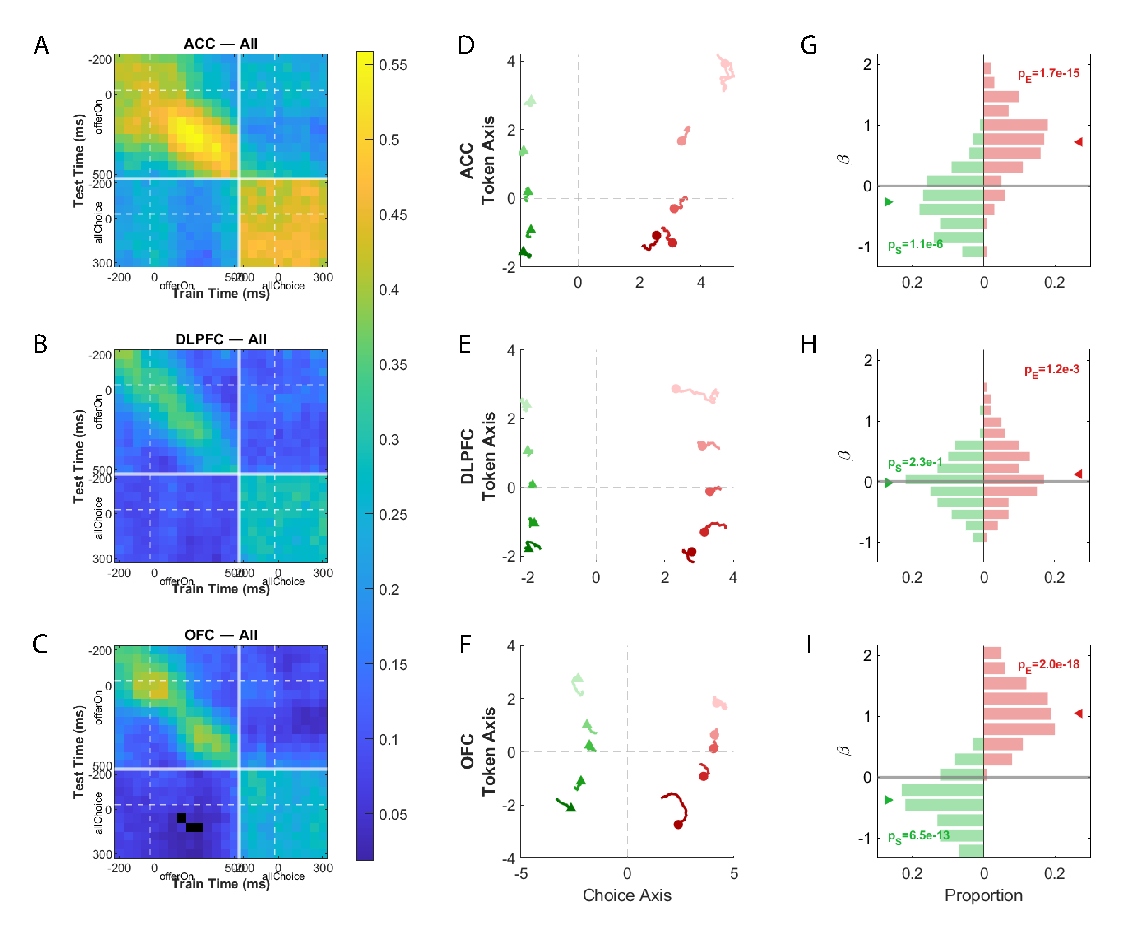
\includegraphics[width=\textwidth]{Figure3_2}
\caption{\textbf{Dynamics of wealth representation.} \textbf{(A--C) Cross-temporal decoding of wealth.} Each entry reports the $R^2$ of wealth decoded using a TDR axis trained at one time bin and tested at another, forming a $24 \times 24$ matrix spanning the offer onset epoch (bins 1--14; 50~ms per bin, $-200$ to $500$~ms relative to offer onset) and the wallet update epoch (bins 15--24; 50~ms per bin, $-200$ to $300$~ms relative to wallet update). Black entries indicate values not significantly exceeding shuffle control (paired rank-sum test, $p > 0.05$). \textbf{(D--F) State-space dynamics during wallet update.} Neural population activity projected into the choice--wealth space derived from TDR ($-100$ to $200$~ms around wallet update). Red and green indicate earning and spending choices, respectively; darker colors correspond to lower wealth levels. Circle and triangle markers indicate the neural state 100~ms prior to choice onset for earning and spending choices, respectively. \textbf{(G--I) Quantification of wealth updates.} Distribution of linear slopes of the wealth-axis projection over time, computed separately for earning (red) and spending (green) choices across bootstrap iterations. Slopes were tested against zero using one-sided Wilcoxon signed-rank tests (right-tailed for earning; left-tailed for spending).}
\label{fig:3_2}
\end{figure}

\subsection{Dynamics of wealth representation}
Beyond the single-unit responses, wealth information was also robustly represented at the population level. To characterize the temporal structure of this representation, we applied cross-temporal decoding: at each time bin, a TDR axis for wealth was fitted independently and then tested at every other bin, yielding a $24 \times 24$ matrix of decoding accuracy ($R^2$) spanning the offer onset and wallet update epochs (Figure~\ref{fig:3_2}A--C). Wealth was decodable even prior to offer onset across all three brain areas, consistent with the wallet remaining visible throughout the ITI. Brain-wise, ACC exhibited stronger wealth decoding across both epochs. [TODO: add brain-wise statistical comparison.]

The structure of the decoding matrix differed between epochs. During the offer onset period, significant decoding was largely confined to entries near the temporal diagonal, while off-diagonal entries were weaker, indicating that the wealth representation evolved continuously and axes trained at one moment transferred poorly to others. On the contrary, decoding accuracy was broadly high across the full wallet update epoch, indicating a representation that generalized stably throughout this period.

Because the direction of wallet updating could be predicted a priori (earning toward greater wealth, spending toward lesser), we examined whether population dynamics during the wallet update reflected a systematic updating of wealth state. Neural activity was projected into the choice--wealth space derived from TDR ($-100$ to $200$~ms around wallet update; Figure~\ref{fig:3_2}D--F). In both ACC and OFC, trajectories exhibited clear choice-dependent shifts: earning choices drove population activity toward the higher-wealth direction, while spending choices drove it toward the lower-wealth direction. To quantify these shifts, we fitted a linear slope to the wealth-axis projection as a function of time, separately for earning and spending choices within each bootstrap iteration. Both ACC and OFC showed significant directional shifts under both choice types (Figure~\ref{fig:3_2}G,~I), whereas the DLPFC showed no such choice-dependent wealth update signal (Figure~\ref{fig:3_2}H).

\begin{figure}[htbp]
\centering
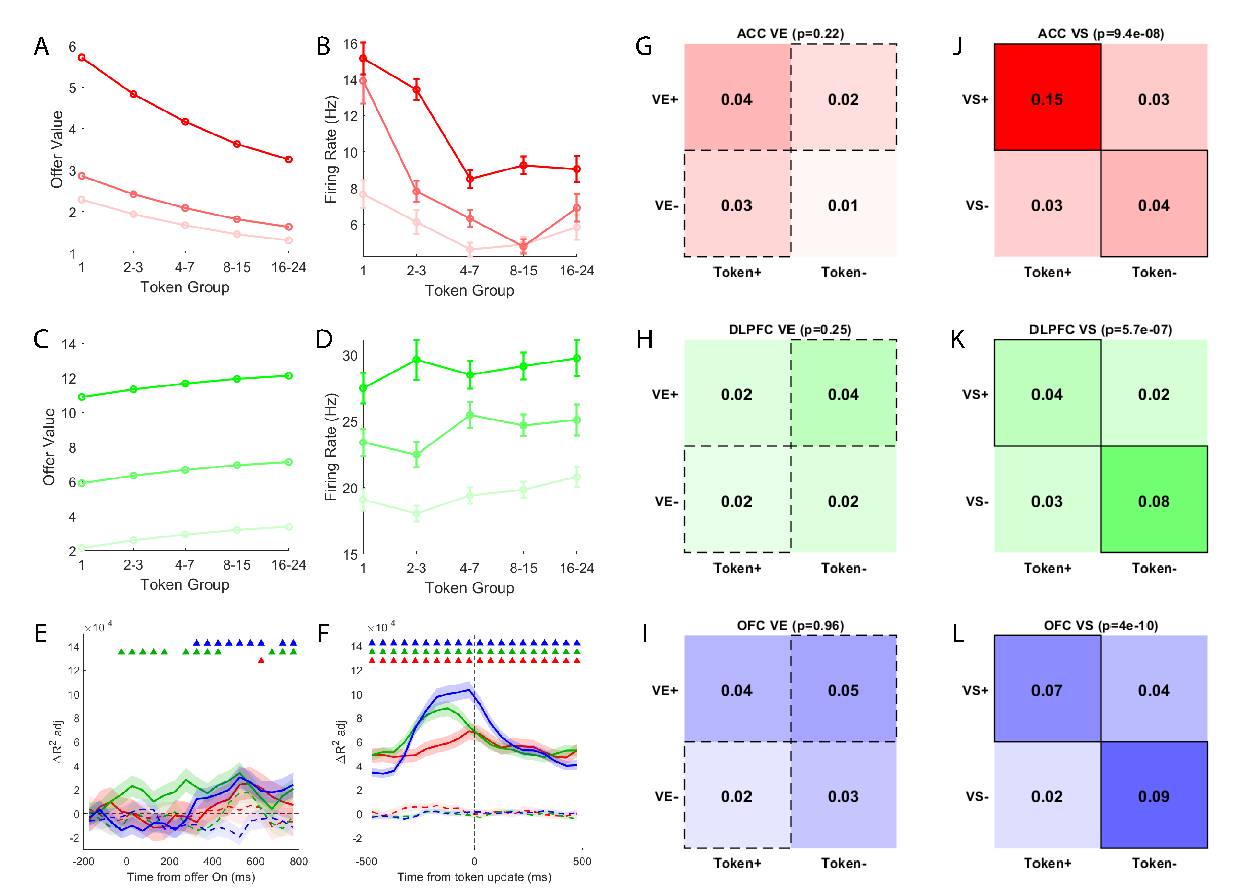
\includegraphics[width=0.75\textwidth]{Figure4}
\caption{
    \textbf{Wealth-Modulated Encoding of Offer Values.} \textbf{(A--D) Representative OFC units encoding offer value.} Tuning curves (mean $\pm$ SEM of firing rate averaged over $-200$ to $300$~ms following token update) as a function of wealth (five token groups, $x$-axis) and offer value (color-coded). Panels (A) and (C) show the theoretical predictions of the behavioral model for earning and spending values, respectively; panels (B) and (D) show representative OFC units whose tuning is modulated by wealth in a manner consistent with these predictions. Darker red indicates higher earning value (A, B); darker green indicates higher spending value (C, D).
    \textbf{(E--F) Time-resolved model comparison ($\Delta R^2$).} Mean of single-unit difference in adjusted $R^2$ between the wealth-modulated model ($M_2$) and the baseline model ($M_1$), aligned to offer onset (E) and wallet update (F). Adjusted $R^2$ was used because $M_1$ and $M_2$ differ in the number of free parameters. Shaded regions indicate $\pm$SEM across units. Colored triangles at the top denote time bins in which $\Delta R^2$ significantly differed from the trial-shuffled null distribution ($p < 0.05$, two-sided Wilcoxon signed-rank test).
    \textbf{(G--I) Joint encoding of earning value and wealth.} $2\times2$ contingency tables showing the proportion of units simultaneously and significantly selective ($p < 0.05$) for both earning value and wealth. A left-tailed Fisher's exact test was applied to test the anti-diagonal pattern ($V_{E,fixed}+$/wealth$-$ and $V_{E,fixed}-$/wealth$+$). No significant directional association was observed in ACC (G), DLPFC (H), or OFC (I).
    \textbf{(J--L) Joint encoding of spending value and wealth.} Same convention as (G--I), but for spending values. A right-tailed Fisher's exact test was applied to test the diagonal pattern ($V_{S,fixed}+$/wealth$+$ and $V_{S,fixed}-$/wealth$-$). Significant associations were found in ACC (J), DLPFC (K), and OFC (L).}
\label{fig:4}
\end{figure}

\subsection{Modulation of Value Encoding by Wealth}
Having established that wealth states are robustly represented in the prefrontal cortex, we next investigated how this economic state modulates the encoding of offer values. Figure~\ref{fig:4}B and D show tuning curves of representative OFC units jointly shaped by offer parameters and wealth level, consistent with the behavioral model predictions (Fig.~\ref{fig:4}A, C).

Because wealth-modulated values derived from the free-$\alpha$ model ($V_E$, $V_S$) and wealth-independent values derived from the fixed-$\alpha$ model ($V_{E,fixed}$, $V_{S,fixed}$) are highly correlated ($r > 0.8$ [TODO: exact number]; see Methods for model details), linear regression produces unstable estimates and cannot reliably distinguish between these variables; we therefore employed joint-encoding analysis as an indirect test. Under the null hypothesis that value and wealth are encoded independently---with no interaction---a unit's selectivity for value and its selectivity for wealth would be randomly associated, producing no systematic diagonal or anti-diagonal pattern in the contingency table. We predicted that spending value encoding should show a diagonal association with wealth encoding ($V_{S,fixed}+$/wealth$+$ and $V_{S,fixed}-$/wealth$-$, where $\pm$ denotes the sign of the regression coefficient): higher wealth reduces the effective cost of spending one token, thereby increasing subjective spending value, so neurons positively encoding spending value should tend to encode wealth positively. For earning, we predicted the opposite anti-diagonal pattern ($V_{E,fixed}+$/wealth$-$ and $V_{E,fixed}-$/wealth$+$): higher wealth reduces the marginal utility of additional tokens, so neurons positively encoding earning value should tend to encode wealth negatively. To test these predictions, we performed a joint-encoding analysis restricted to units simultaneously and significantly selective ($p < 0.05$) for both offer values and wealth. Directional Fisher's exact tests were then applied to assess the predicted associative patterns. The diagonal pattern for spending was confirmed across all three PFC regions (Fig.~\ref{fig:4}J--L). No significant directional association was found for earning in any region (Fig.~\ref{fig:4}G--I), though this null result may partly reflect limited statistical power, as earning-selective neurons were less prevalent than spending-selective neurons across all three regions.

We further examined the specific contribution of wealth modulation to earning value encoding using a model comparison approach. The baseline model ($M_1$) included wealth-independent values ($V_{E,fixed}$, $V_{S,fixed}$), choice, and wealth; wealth was treated as a categorical variable, captured by dummy variables to non-parametrically absorb any arbitrary function of token level. The wealth-modulated model ($M_2$) extended $M_1$ with a single additional regressor, $V_E$, which is a multiplicative interaction between earning rate and wealth and cannot be absorbed by the wealth dummy variables or $V_{E,fixed}$ in $M_1$ separately. By contrast, the wealth-modulated spending value takes an additive form that is exactly collinear with the combination of $V_{S,fixed}$ and the wealth dummies in $M_1$, and would therefore contribute no additional explanatory power; accordingly, it was not included in this analysis. We found that $\Delta R^2 = R^2_2 - R^2_1$ was significantly positive across all three PFC regions during the wallet update epoch (Fig.~\ref{fig:4}F) but not during offer onset (Fig.~\ref{fig:4}E). Taken together, these results confirm that wealth systematically modulates the neural encoding of offer values across prefrontal subregions.

\begin{figure}[htbp]
\centering
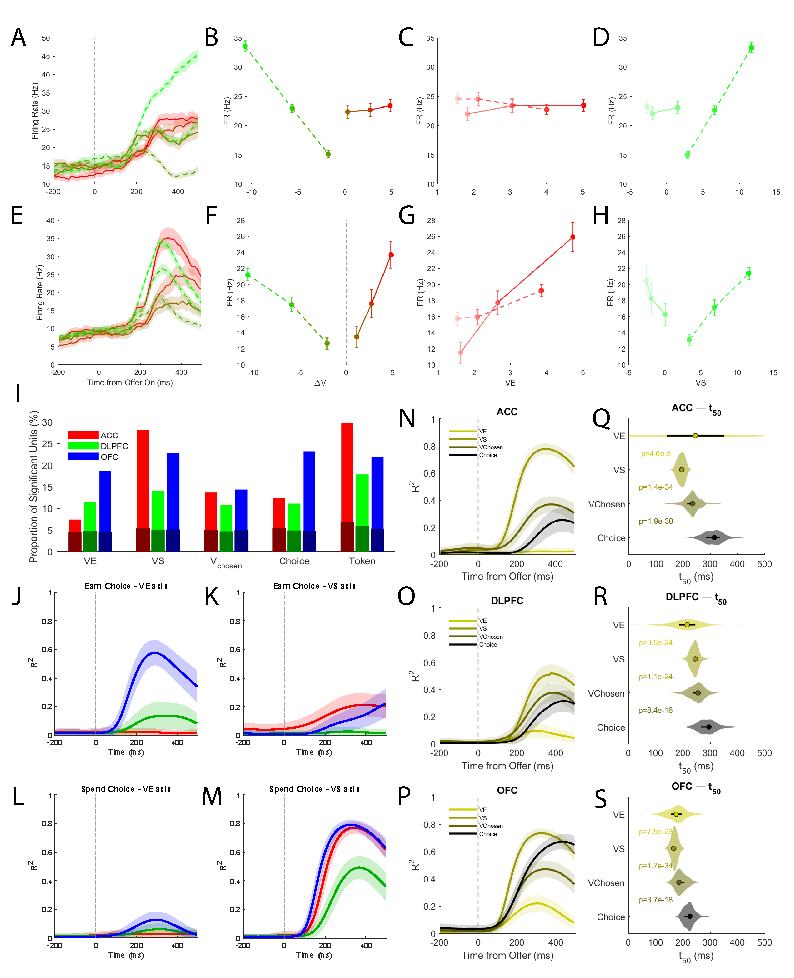
\includegraphics[width=0.72\textwidth]{Figure5}
\caption{\textbf{Encoding of the Chosen Value.} \textbf{(A--H) Representative units encoding $V_{\mathrm{Chosen}}$.} \textbf{(A) and (E):} Peri-stimulus time histograms (PSTHs) aligned to offer onset. Solid and dashed lines indicate earning and spending choices, respectively. The color gradient from red to green represents the transition from high (favoring earning) to low (favoring spending) $\Delta V$. \textbf{(B) and (F):} Tuning curves grouping trials by choice and $\Delta V$ tertile. Each choice type was split into three tertiles of $\Delta V$; same color gradient as in (A) and (E). \textbf{(C) and (G):} Tuning curves grouping trials by choice and $V_E$ tertile. The color gradient from light to dark red represents low to high $V_E$ within each choice condition. \textbf{(D) and (H):} Tuning curves grouping trials by choice and $V_S$ tertile. The color gradient from light to dark green represents low to high $V_S$ within each choice condition. \textbf{(I) Proportion of units encoding task-related variables.} Five variables ($V_E$, $V_S$, $V_{\mathrm{Chosen}}$, Choice, Wealth) were included simultaneously in a single regression model ($\alpha = 0.05$). Light bars show the proportion of significantly encoding units; dark overlaid bars indicate chance level. Red, green, and blue denote ACC, DLPFC, and OFC, respectively. \textbf{(J--M) Choice-conditioned TDR.} TDR analysis was performed separately within earning (J, K) and spending (L, M) trial pools. Encoding strength ($R^2$) of $V_E$ (J, L) and $V_S$ (K, M) was higher when the variable corresponded to the chosen option (congruent: J and M) than when it did not (incongruent: K and L). Shaded regions indicate $\pm$1 SD across 100 bootstrap permutations. \textbf{(N--P) Comparison of $V_E$, $V_S$, $V_{\mathrm{Chosen}}$, and Choice encoding strength.} TDR was performed separately for all four variables. Encoding strength $R^2(t)$ is plotted for each variable and brain area: ACC (N), DLPFC (O), and OFC (P). Shaded regions indicate $\pm$1 SD across 100 bootstrap permutations. \textbf{(Q--S) Temporal dynamics of encoding.} For each $R^2(t)$ trajectory, $t_{50}$ was defined as the first time point in $[0, T_{\mathrm{peak}}]$ at which $R^2$ exceeded the midpoint between the pre-stimulus baseline median and the peak value, provided the peak was significant (one-sided, 95th percentile of the baseline distribution). Violin plots show the $t_{50}$ distribution across 100 bootstrap permutations per brain area (ACC: Q, DLPFC: R, OFC: S); violin area is proportional to the fraction of permutations yielding a valid estimate. Horizontal lines denote the median and interquartile range. P values from pairwise Wilcoxon rank-sum tests comparing each value variable against the choice signal are displayed to the left when the value signal preceded choice $(t_\text{value} < t_\text{choice})$, to the right when choice preceded the value signal $(t_\text{choice} < t_\text{value})$, and centered when no significant difference was detected.}
\label{fig:5}
\end{figure}

\subsection{Encoding of the Chosen Value}
The value difference $\Delta V = V_E - V_S$ is a continuous analogue of the binary choice, making it a natural candidate for driving that choice. We therefore first asked whether $\Delta V$ constitutes a dominant encoding feature at the single-unit level. Because $\Delta V$ is an exact linear combination of $V_E$ and $V_S$, linear regression cannot distinguish a unit genuinely encoding the difference from a unit with mixed selectivity for $V_E$ and $V_S$. We instead applied a joint-encoding analysis (similar to Fig.~\ref{fig:4}G--L) to units that showed significant tuning to both $V_E$ and $V_S$, testing whether co-encoding units were disproportionately concentrated in the anti-diagonal cells (i.e., $V_{E,\mathrm{pos}} \times V_{S,\mathrm{neg}}$ or $V_{E,\mathrm{neg}} \times V_{S,\mathrm{pos}}$), as would be expected for a true $\Delta V$ representation. Fisher's exact tests revealed no significant anti-diagonal pattern in any of the three brain areas (Figure~S11), indicating that $\Delta V$ encoding is not a dominant feature at the single-unit level.

What single units encoded instead was the value of the chosen option---whichever option the animal selected on that trial. We identified units whose value tuning was systematically modulated by the animal's choice (Figure~\ref{fig:5}A--H). A representative unit (Figure~\ref{fig:5}A--D) encoded $V_S$ only during spending choices and was unresponsive to $V_E$. The second representative unit (Figure~\ref{fig:5}E--H) encoded both $V_E$ and $V_S$, but with choice-dependent sensitivity: $V_S$ tuning was positive during spending choices yet reversed sign during earning choices, while the slope of $V_E$ tuning was steeper during earning choices than during spending choices. These units are analogous to $V_{\mathrm{Chosen}}$ cells originally described in the orbitofrontal cortex~\cite{padoa-schioppaNeuronsOrbitofrontalCortex2006b}. Linear regression confirmed that the proportion of units significantly encoding $V_{\mathrm{Chosen}}$ exceeded chance levels in all three areas (Figure~\ref{fig:5}I).

To verify this choice-dependent value representation at the population level, we performed choice-conditioned TDR, fitting value axes separately within earning and spending trial pools (Figure~\ref{fig:5}J--M). Encoding of $V_E$ was substantially stronger during earning choices than during spending choices (Figure~\ref{fig:5}J, L), and the complementary pattern held for $V_S$ (Figure~\ref{fig:5}K, M). This asymmetry between congruent and incongruent signals indicates that choice-dependent value encoding is a prominent feature of prefrontal population activity.

The $V_{\mathrm{Chosen}}$ signal could either precede and drive the choice or arise as a downstream consequence of it. We addressed this question by comparing the temporal emergence of value and choice signals in TDR analyses (Figure~\ref{fig:5}N--P). In all three regions, $V_E$, $V_S$, and $V_{\mathrm{Chosen}}$ signals all reached their half-peak amplitude ($t_{50}$) significantly earlier than the choice signal (pairwise Wilcoxon rank-sum tests; Figure~\ref{fig:5}Q--S; see Figure~S14 for a complementary onset latency analysis, defined as the first time point exceeding the pre-stimulus baseline), arguing against the possibility that $V_{\mathrm{Chosen}}$ merely reflects a decision already made.

Together, these results demonstrate that all three prefrontal regions encode $V_{\mathrm{Chosen}}$, a signal that bridges value computation and behavioral choice. Among these regions, OFC exhibited the broadest value encoding profile, with significant signals for $V_E$, $V_S$, and $V_{\mathrm{Chosen}}$ (Figure~S15), supporting its role as a key integrative node for wealth-modulated offer values.

\section{Methods}\label{sec3}

\subsection{Subjects and Materials}
Three naive male rhesus monkeys (\textit{Macaca mulatta}; monkeys W, U, and T) were used in this study, weighing between 4 and 6 kg during the experiments. All procedures were approved by the Animal Care Committee of Shanghai Institutes for Biological Sciences, Chinese Academy of Sciences (Shanghai, China). During each experimental session, monkeys were seated in a primate chair facing a 23.6-inch video monitor positioned 60 cm away. Eye position was monitored at 1000 Hz using an infrared oculometer (EyeLink 1000). Water reward was delivered via a computer-controlled solenoid valve, with monkeys consuming approximately 200 mL per session.

\subsection{Behavioral task}
Monkeys were trained on a novel earning--spending task (Figs.~\ref{fig:1}A,~B). Each trial began with the simultaneous onset of two stimuli representing earning and spending options, positioned diametrically opposite at $6^\circ$ eccentricity; target locations were drawn from a uniform distribution over $[0, 2\pi]$ on each trial. Monkeys indicated their choice by fixating on a target for a required duration. For spending choices, one token was deducted per 200 ms of continuous fixation (5 tokens/s). For earning choices, tokens were added individually at rates corresponding to the offer's $V_\text{Earn}$: 250, 200, or 100 ms per token (4, 5, or 10 tokens/s, respectively).

Wealth was represented by a central ``wallet'' ($5 \times 5$ array of circles, $4^\circ$ in side length) that updated in real time. Tokens accumulated across trials and were only removed upon spending. To maintain a continuous representation of wealth, the wallet remained visible during the inter-trial interval (ITI, ${\sim}1$ s) while choice stimuli were absent. Trial durations were sampled from an exponential distribution to minimize temporal anticipation. Each session began with 0 tokens.

\subsection{Training}
Following acquisition of a standard delayed saccade task, monkeys were progressively trained on the earning--spending task. Reward magnitude ($V_\text{Spend}$) was initially set high to ensure adequate daily water intake, then gradually reduced as each monkey's choice behavior converged to a stable pattern. Full training was completed in approximately 6 months for all subjects.

\subsection{Surgery}
Prior to task training, each monkey received a chronic titanium headpost implant under standard sterile surgical conditions. Following behavioral stabilization, a second surgery was performed to implant an acrylic recording chamber over the prefrontal cortex, centered over the principal sulcus, with a craniotomy made within the chamber (inner dimensions: $19.5 \times 24$ mm). All surgeries were conducted under aseptic conditions. Monkeys were sedated with ketamine hydrochloride (5-15 mg/kg, i.m.) and maintained under isoflurane anesthesia (1.5-2\%, to effect); heart rate, blood pressure, body temperature, and end-tidal CO$_2$ were monitored continuously throughout.

\subsection{MRI}
Structural MRI scans were acquired before and after chamber implantation using a Siemens 3T scanner to identify and verify recording locations. Monkeys were sedated with ketamine hydrochloride (5--15 mg/kg, i.m.) and maintained under isoflurane anesthesia (1.5--2\%, to effect) during scanning.

\subsection{Behavioral analysis}

\subsubsection{Non-parametric weight estimation}
To quantify the modulation of option value by wealth without assuming a specific functional form, we estimated subjective weights for the seven shapes (three earning, four spending) at each of the 24 wealth levels. Earning probability was modeled by a sigmoid function:
\begin{equation}
P_\text{earn} = \frac{1}{1 + \exp\!\bigl(-(V_{e,w} - V_{s,w})\bigr)},
\end{equation}
where $V_{e,w}$ and $V_{s,w}$ are the estimated weights of the earning and spending options at wealth level $w$. To regularize the solution and encourage gradual variation across wealth levels, we augmented the cross-entropy loss with an $L_2$ smoothing penalty on differences between adjacent wealth levels:
\begin{align}
L = & -\sum_{i} \bigl[c_i \ln \hat{p}_i + (1 - c_i) \ln(1 - \hat{p}_i)\bigr] \\
& + \lambda \sum_{e,s,w} \bigl(V_{e/s,w} - V_{e/s,w+1}\bigr)^2,
\end{align}
where $c_i \in \{0,1\}$ is the binary choice (1 = earn, 0 = spend), $\hat{p}_i$ is the predicted earning probability, and $\lambda = 10$ controls the smoothing strength. Parameters were estimated by unconstrained optimization (\texttt{fminunc}, quasi-Newton algorithm, MATLAB).

\subsubsection{Parametric utility model}
We developed a parametric model based on marginal utility theory. We assumed a power-law utility function $U(w) = w^\alpha$, where $w$ denotes the current wealth (accumulated tokens) and $\alpha$ is the curvature exponent. The subjective values of earning and spending were defined as:
\begin{align}
V_\text{Earn} &= \frac{ES}{ER} \cdot \alpha w^{\alpha-1}, \\
V_\text{Spend} &= R \cdot SS - \frac{SS}{ER} \cdot \alpha w^{\alpha-1},
\end{align}
where $ES$ is the earning speed (tokens/s), $R$ is the normalized reward magnitude (in arbitrary units), $ER$ is the exchange rate (tokens per unit reward), and $SS = 5$ tokens/s is the spend speed. The first term in $V_\text{Spend}$ represents the immediate reward benefit; the second captures the opportunity cost of spending a token scaled by its marginal utility. The integrated decision variable was $V_\text{total} = V_\text{Earn} - V_\text{Spend}-\text{bias}$, and choice probability was given by:
\begin{equation}
P_\text{earn} = \frac{1}{1 + \exp\!\left(-\dfrac{V_\text{total}}{\gamma}\right)},
\end{equation}
where $\gamma > 0$ is the choice sensitivity and $\text{bias}$ is a decision bias. Free parameters $(\alpha,\, ER,\, \text{bias},\, \gamma)$ were estimated by minimizing the cross-entropy loss using \texttt{fmincon} (SQP algorithm, MATLAB) with MultiStart (10 random initializations) to mitigate convergence to local optima.

The \textit{fixed-$\alpha$} model served as a nested baseline in which $\alpha$ was constrained to 1, corresponding to linear marginal utility. All remaining parameters were estimated freely, allowing direct assessment of whether wealth-dependent curvature in utility is necessary to account for the observed choice patterns.

\subsubsection{Leave-one-session-out cross-validation}
To evaluate out-of-sample predictive performance, we applied leave-one-session-out (LOSO) cross-validation. In each fold, model parameters were estimated on the pooled data from all remaining sessions (training set) and evaluated on the held-out session (test set). Model performance on the held-out session was quantified as the average negative log-likelihood per trial (NLL/trial). The per-fold loss difference was defined as $\Delta L = L_\text{fixed} - L_\text{free}$, so that positive values indicate better generalization of the free-$\alpha$ model. Statistical significance was assessed using the Wilcoxon signed-rank test across folds.

\subsubsection{Session-wise $\alpha$ estimation}
To characterize the distribution of the marginal utility exponent $\alpha$ across recording sessions, the free-$\alpha$ model was fitted independently to each session's data. The exponent was constrained to the interval $[0, 1]$ by construction. Per-session $\alpha$ estimates were pooled within each subject and displayed as histograms with a bin width of 0.05. To test whether $\alpha$ deviated significantly from linear marginal utility, a Wilcoxon signed-rank test was applied against the null hypothesis $\alpha = 1$ for each subject.

\subsection{Electrophysiology}
Neuronal activity was recorded using 16-channel linear array electrodes (Plexon S-probe) and acquired with an AlphaLab SnR system (AlphaOmega). Electrodes were driven by a multichannel micromanipulator (Alpha Omega EPS). Spike sorting was performed automatically using Kilosort4; each unit was subsequently truncated to epochs of sustained activity (firing rate $> 1$ Hz within a 60 s sliding window). In total, we recorded 679 units from the ACC (247 and 432 from monkeys W and T, respectively; monkey U had no ACC recordings), 1,056 units from the DLPFC (127, 491, and 438 for monkey W, U, and T, respectively), and 903 units from the OFC (111, 446, and 346 for monkey W, U, and T, respectively). Based on MRI reconstructions and physiological landmarks observed during electrode penetrations, ACC recordings corresponded approximately to BA 24, OFC to BA 11, and DLPFC to BA 46 (SI Appendix, Fig.~S2).

\subsection{Representative neuron peristimulus time histograms (PSTHs)}
Firing rates for the illustrated units were computed by convolving spike trains with a causal Gaussian kernel ($\sigma = 100$~ms; half-window = 300~ms). The causal kernel spans only the interval $[-300, 0]$~ms relative to each time point, ensuring that the smoothed rate at any moment depends exclusively on preceding spikes and introduces no forward leaking.

\subsection{Choice Selectivity}
For each neuron, firing rates were averaged over the offer period (0--500~ms post-onset) to yield a single response scalar per trial. These mean rates were regressed against the monkey's binary choice in each domain:
\begin{equation}
FR \sim \beta_0 + \beta_1 \cdot Choice_{LR} + \beta_2 \cdot Choice_{ES}
\end{equation}
The resulting $p$-values quantified each unit's selectivity in the action ($p_{LR}$) and good-based ($p_{ES}$) domains (Figure~\ref{fig:2}C). Area-level preferences were assessed by comparing the proportion of neurons satisfying $p_{ES} < p_{LR}$ against chance using a two-sided binomial test.

\subsection{Targeted Dimensionality Reduction (TDR)}
We employed TDR to project population firing patterns into a low-dimensional subspace aligned to task-relevant variables.

\subsubsection{Unit Filtering}
Neurons were filtered based on the requirements of each analysis. For the primary TDR analyses, a unit was retained if it contributed at least 50 valid trials in total, with a minimum of 10[TBD] trials per condition group.

\subsubsection{Regression}
Firing rates at each time bin were z-scored independently: the mean and standard deviation across training trials were computed at each time bin and applied to normalize both training and test responses, preventing test-set information from entering the fitted model. Task variables were likewise z-scored within the training partition. The regression target for each neuron was the z-scored firing rate averaged over the analysis-specific regression window, yielding one scalar observation per trial. Ordinary least squares (OLS) regression was then applied to estimate each neuron's coefficient vector $\boldsymbol{\beta}_n \in \mathbb{R}^{V}$; these were stacked row-wise to form the population coefficient matrix $\mathbf{B} \in \mathbb{R}^{N \times V}$.

For the results in Figures~\ref{fig:2}, we used the following model (regression window: 0--500~ms aligned to offer onset; projection window: -200--500~ms):
\begin{equation}
FR \sim \sum_v \beta_v V_v + \beta_{w}\,Wealth + \sum_c \beta_c Choice_c + \beta_0
\end{equation}
where $V_v \in \{V_L, V_R, V_E, V_S\}$ denote the values of the spatially-mapped and task-defined options, $Wealth$ is the accumulated token count at offer onset, and $Choice_c \in \{Choice_{LR}, Choice_{ES}\}$ represents the monkey's choices in the action and good-based domains. Because $V_L$/$V_R$ and $V_E$/$V_S$ are collinear by construction, ridge regression ($\lambda = 5$) replaced OLS for this model to stabilize coefficient estimation; all other models used standard OLS.

For the results in Figure~\ref{fig:3_2} (regression window: $-100$--200~ms relative to token update; projection window: $-100$--200~ms):
\begin{equation}
FR \sim \beta_0 + \beta_1\,V_E + \beta_2\,V_S + \beta_3\,Choice_{ES} + \beta_4\,Wealth
\end{equation}

To isolate value encoding from choice-related activity (Figure~\ref{fig:5}J--M), trials were partitioned by the monkey's behavioral output (earning vs.\ spending) and independent TDR models were fit within each condition (regression window: 0--500~ms post-offer; projection window: $-200$--500~ms):
\begin{equation}
FR \sim \beta_0 + \beta_1\,V_E + \beta_2\,V_S + \beta_3\,Wealth
\end{equation}
The coefficient matrix was orthogonalized via QR decomposition with column ordering $[\boldsymbol{\beta}_{Wealth},\, \boldsymbol{\beta}_{V_E},\, \boldsymbol{\beta}_{V_S}]$, yielding encoding axes for $V_E$ and $V_S$ residualized against wealth effects. Test trials were stratified into tertiles of the corresponding value variable (100 trials per tertile). The analysis was repeated over 100 bootstrap iterations, each resampling units with replacement (100 per individual subject; 300 for the pooled analysis).

To compare the temporal emergence of value and choice signals (Figure~\ref{fig:5}N--P), a joint model was fit over the offer-onset epoch (regression window: 0--500~ms; projection window: $-200$--500~ms):
\begin{equation}
FR \sim \beta_0 + \beta_1\,Wealth + \beta_2\,Choice + \beta_3\,V_E + \beta_4\,V_S + \beta_5\,V_{\mathrm{Chosen}}
\end{equation}
Four separate encoding axes were extracted by repeating QR decomposition with the target variable placed last in the column ordering, ensuring each axis is orthogonal to all others. Test trials were stratified into two groups for the choice axis (150 trials per group) or three tertile groups for value axes (100 trials per group).

\subsubsection{Orthonormalization and Projection}
The coefficient matrix $\mathbf{B}$ was orthonormalized via QR decomposition:
\begin{equation}
\mathbf{B} = \mathbf{Q}\mathbf{R}
\end{equation}
where the columns of $\mathbf{Q} \in \mathbb{R}^{N \times V}$ form an orthonormal basis of task-related population axes. Task variables were ordered so that the target variable occupied the final column, ensuring that its corresponding axis was residualized against all other regressors. Time-resolved population signals were then obtained by projecting the z-scored test-set firing rate matrix $\mathbf{X}(t)$ at each time point onto this basis:
\begin{equation}
\mathbf{P}(t) = \mathbf{Q}^T \mathbf{X}(t)
\end{equation}

\subsubsection{Cross-Validation}
To obtain stable estimates of encoding strength and characterize their uncertainty, the regression--projection pipeline was repeated over $N_{CV}$ (10 for cross-temporal decoding and 100 for other TDR analyses) bootstrap iterations. In each iteration, neurons were resampled with replacement from the full pool (100 per individual subject; 300 for the pooled analysis), and a fresh 50/50 trial partition was drawn independently per unit. The resampled training set was used to fit $\mathbf{B}_p$ and derive the corresponding orthonormal axes $\mathbf{Q}_p$; test-set firing rates were then projected onto $\mathbf{Q}_p$. To evaluate encoding strength, test trials were assigned to condition groups (e.g., earning vs.\ spending for the ES axis; left vs.\ right for the LR axis) and resampled with replacement. Regardless of the number of groups, a fixed total of 300 trials were drawn---distributed evenly across groups (e.g., 150 trials per group for 2-group comparisons; 100 per group for 3-group comparisons)---and pooled with their corresponding labels into a single vector. Encoding strength at each time point was then quantified as the squared Pearson correlation between the pooled projection and the group labels:
\begin{equation}
R^2(t) = \left[\mathrm{corr}\!\left(\mathbf{p}(t),\, \mathbf{l}\right)\right]^2
\end{equation}
where $\mathbf{p}(t)$ is the vector of pooled projections at time $t$ and $\mathbf{l}$ the corresponding group label vector. The mean and standard deviation of $R^2(t)$ across $N_{CV}$ iterations are reported throughout.

\subsubsection{Cross-Temporal Decoding}
To assess the temporal stability of encoded variables across task epochs, we performed cross-temporal decoding for both token wealth and the value variables ($V_E$, $V_S$, $V_{\mathrm{Chosen}}$). Time bins were defined at 50~ms resolution. For token wealth, 14 bins spanned the offer-onset epoch ($-200$ to $500$~ms) and 10 bins spanned the wallet-update epoch ($-200$ to $300$~ms), yielding a $24 \times 24$ decoding matrix; for the value variables, 10 bins spanned the offer-onset epoch ($0$ to $500$~ms) and 10 bins the peri-choice epoch ($-200$ to $300$~ms), yielding a $20 \times 20$ matrix. At each training bin, a TDR axis was fitted following the regression and QR orthogonalization procedures described above and used to decode the target variable at every other bin, with $R^2$ computed from tertile-stratified test trials. The procedure was repeated for $N_{CV} = 10$ bootstrap iterations; the reduced number of iterations reflects the computational cost of the full cross-temporal design. In each iteration, units were resampled without replacement (100 per individual subject; 300 for the pooled analysis) and a fresh trial partition was drawn independently per unit. The mean $R^2$ across iterations is reported.

Each matrix entry was tested against a shuffle control in which variable labels were permuted across trials within each unit. Statistical significance was assessed using a one-sided Wilcoxon signed-rank test comparing real and shuffle $R^2$ values across bootstrap iterations. Entries not significantly exceeding the shuffle distribution are displayed in black.

\subsubsection{Latency Analysis}
Two latency metrics were derived from each $R^2(t)$ trajectory. The \emph{raising time} was defined as the onset of the first sustained cluster of $R^2$ values exceeding the 95th percentile of the pre-stimulus baseline distribution (constructed from $R^2$ in $[-200, 0)$~ms); a cluster was required to span at least five consecutive time bins ($\geq 25$~ms). The \emph{half-peak time} ($t_{50}$) was defined as the first time point in $[0, T_{\mathrm{peak}}]$ at which $R^2(t)$ reached the midpoint between the baseline median and the response peak $R_{\mathrm{max}}$; permutations for which $R_{\mathrm{max}}$ did not exceed the baseline 95th percentile were assigned $t_{50} = \mathrm{NaN}$ and excluded. Raising time and $t_{50}$ were each compared across variables using pairwise two-sided Wilcoxon rank-sum tests ($V_E$, $V_S$, and $V_{\mathrm{Chosen}}$ each against the choice signal). Violin plots show the kernel density estimate (reflection boundary correction) of valid values across 100 bootstrap permutations; violin width is proportional to the fraction of permutations yielding a valid estimate.

\subsection{Wealth Selectivity}
To quantify wealth selectivity, we regressed the mean firing rate in a window of $-300$ to $300$~ms relative to offer onset against task variables:
\begin{equation}
    FR \sim \beta_1 V_E + \beta_2 V_S + \beta_3 Choice_{ES} + \beta_4 Wealth + \beta_0
    \label{eq:cat_wealth}
\end{equation}
where $Wealth$ denotes the subject's accumulated token count at offer onset, treated as a categorical variable with five levels ([1], [2--3], [4--7], [8--15], [16--24]). A logarithmic binning scheme was used to define these levels, ensuring a balanced number of trials across categories and accounting for the natural distribution of wealth states encountered during the task. Neurons were classified as wealth-selective if the $F$-test for the $Wealth$ term reached significance ($\alpha = 0.05$). The preferred wealth level was defined as the level yielding the smallest $p$-value across pairwise two-sample $t$-tests, each comparing the mean firing rate of one wealth group against all remaining groups combined. The direction of tuning was determined by the sign of $\bar{r}_{pref} - \bar{r}_{rest}$. For population averaging, the tuning curves of negatively tuned neurons ($\bar{r}_{pref} - \bar{r}_{rest} < 0$) were inverted prior to normalization. Min-max normalization was then applied:
\begin{equation}
    TC_{norm} = \frac{TC - \min(TC)}{\max(TC) - \min(TC)}
\end{equation}
Normalized curves were averaged across neurons sharing the same preferred wealth level to yield group-level population tuning curves. To characterize the shape of the re-centered population tuning curves (Fig.~\ref{fig:3_1}I--K), the normalized firing rates at relative positions $\pm1$ and $\pm2$ from each neuron's preferred wealth level were extracted and compared using a Wilcoxon rank-sum test. Under the null hypothesis that the tuning curves reflect random noise, firing rates at all non-peak positions would be indistinguishable from one another; a significant difference between positions $\pm1$ and $\pm2$ therefore provides evidence for a genuine, graded decay away from the response peak. This interpretation is corroborated by a shuffle control (Fig.~S6), in which wealth group labels were randomly permuted across trials prior to all analyses, confirming that the observed gradient structure cannot be attributed to chance.

\subsection{Offer Value Selectivity and Wealth Modulation}

\subsubsection{Firing rate estimation}
Spike trains were smoothed with a causal Gaussian kernel ($\sigma = 10\,\mathrm{bins}$). For the time-resolved model comparison, smoothed firing rates were subsequently averaged within non-overlapping 50\,ms bins spanning $-200$ to $800\,\mathrm{ms}$ relative to offer onset and $-500$ to $500\,\mathrm{ms}$ relative to wealth update.

\subsubsection{Time-resolved model comparison}
Two nested linear models were fitted at each 50\,ms time bin. The baseline model ($M_1$) incorporated objective offer values, choice direction, and 23 binary wealth-level dummy variables (one indicator per wealth value 2--24, with wealth=1 token as the reference level):
\begin{equation}
\mathrm{FR} \sim \beta_0 + \sum_i\beta_i V_i^{\mathrm{obj}} + \beta_3\,\mathrm{Choice} + \sum_{k=2}^{24} \gamma_k\,\mathbf{1}[\mathrm{Wealth} = k].
\end{equation}
where $V_i^{\mathrm{obj}}$ includes the objective earning and spending values derived from the fixed-$\alpha$ behavioral model. The wealth-modulated model ($M_2$) extended $M_1$ with the free-$\alpha$ earning value as an additional regressor:
\begin{align}
\mathrm{FR} \sim & \beta_0 + \sum_i\beta_i V_i^{\mathrm{obj}} + \beta_3\,\mathrm{Choice} + \sum_{k=2}^{24} \gamma_k\,\mathbf{1}[\mathrm{Wealth} = k] \\
& + \beta_4\,V_{E,w}.
\end{align}
Model performance was quantified by adjusted $R^2$ to penalise the additional free parameter in $M_2$. The wealth modulation index $\Delta R^2 = R^2_{\mathrm{adj}}(M_2) - R^2_{\mathrm{adj}}(M_1)$ was computed per unit at each time bin. At each bin, the significance of the population-level $\Delta R^2$ was assessed using a two-sided Wilcoxon signed-rank test comparing per-unit $\Delta R^2$ values against those obtained from a trial-shuffled null, in which the rows of each unit's firing-rate matrix were randomly permuted to destroy all stimulus--response associations while preserving the covariance structure of the regressors.

\subsubsection{Joint-encoding analysis}
To characterise the co-representation of offer value and wealth, the following regression was fitted to each unit's mean firing rate over 0--150\,ms following wealth update:
\begin{equation}
\mathrm{FR} \sim \beta_0 + \sum_i\beta_i V_i^{\mathrm{obj}} + \beta_3\,\mathrm{Choice} + \beta_4\,\mathrm{Wealth},
\end{equation}
where wealth was entered as a continuous linear predictor and objective (fixed-$\alpha$) values were used to ensure that the wealth coefficient captured wealth-related firing variance orthogonal to value encoding. A unit was classified as positively or negatively selective for a given variable if the corresponding regression coefficient was significant ($p < 0.05$); otherwise it was excluded from the contingency for that variable pair. Only units simultaneously selective for both value and wealth were entered into the $2\times2$ contingency table. For earning value, a left-tailed Fisher's exact test was applied, based on the a priori directional prediction that diminishing marginal utility produces an anti-diagonal pattern (VE$+$/Token$-$). For spending value, a right-tailed Fisher's exact test was used, reflecting the complementary prediction that higher wealth increases subjective spending value, producing a diagonal pattern (VS$+$/Token$+$).

\subsection{$\Delta V$ Selectivity}
To test whether single units preferentially encoded the value difference $\Delta V = V_E - V_S$, we fit an OLS regression model to mean firing rates in the offer-onset epoch ($[0, 500]$~ms) and the token-update epoch ($[0, 150]$~ms):
\begin{equation*}
    \mathrm{FR} \sim \beta_0 + \beta_1 V_E + \beta_2 V_S + \beta_3 \, \mathrm{Choice} + \sum_{k=2}^{24} \gamma_k \, \mathbf{1}[\mathrm{token} = k],
\end{equation*}
where token wealth was included as a 23-level dummy-coded categorical variable (token 1 as reference). A unit was classified as $V_E$-positive ($V_{E,\mathrm{pos}}$) if $\beta_1 > 0$ and $p(\beta_1) < 0.05$, as $V_E$-negative ($V_{E,\mathrm{neg}}$) if $\beta_1 < 0$ and $p(\beta_1) < 0.05$, and non-selective otherwise; the analogous classification was applied to $\beta_2$ for $V_S$. Among units significant for both $V_E$ and $V_S$, we constructed a $2 \times 2$ contingency table (rows: $V_E$ sign; columns: $V_S$ sign) and applied Fisher's exact test to assess whether the anti-diagonal cells ($V_{E,\mathrm{pos}} \times V_{S,\mathrm{neg}}$ and $V_{E,\mathrm{neg}} \times V_{S,\mathrm{pos}}$) were over-represented, as would be expected if $\Delta V$ were the dominant encoded quantity.

\subsection{$V_{\mathrm{Chosen}}$ selectivity}
The behavioral model includes a bias parameter $b$ representing the animal's indifference point between earning and spending. This parameter enters the choice rule as a shift on $V_E - V_S$ and cannot be attributed to either offer value independently; partitioning it between $\beta_{V_E}$ and $\beta_{V_S}$ would be arbitrary. We therefore defined a composite variable
\begin{equation*}
    V_{\mathrm{Chosen}} = (V_E - V_S - b) \times c,
\end{equation*}
where $c = +1$ for earning choices and $c = -1$ for spending choices. This formulation captures the value advantage of the chosen option relative to the animal's subjective indifference point in a single coefficient. The regression model was
\begin{equation*}
    \mathrm{FR} \sim \beta_0 + \sum_i\beta_i V_i + \beta_4 \, \mathrm{Choice} + \sum_{k=2}^{24} \gamma_k \, \mathbf{1}[\mathrm{token} = k],
\end{equation*}
where $V_i\in\{V_E,V_S,V_{Chosen}\}$, fit to mean firing rates in the offer-onset epoch ($[0, 500]$~ms). Token wealth was treated as a categorical predictor; its significance was assessed via a partial $F$-test from model ANOVA. Units with $p(\beta_3) < 0.05$ were classified as $V_{\mathrm{Chosen}}$-selective. The proportion of selective units per area was compared against a chance level estimated by repeating the regression 10 times with randomly permuted firing rates and averaging the resulting false-positive proportions.

\section{Discussion}\label{sec4}

We introduce the earning--spending task, a novel paradigm in which macaques chose, on every trial, between acquiring tokens and spending accumulated tokens for immediate juice reward---to our knowledge, the first task to record prefrontal electrophysiology during wealth-dependent earning and spending decisions in non-human primates. Consistent with diminishing marginal utility, all three animals showed systematic shifts in preference as a function of accumulated wealth. At the neural level, three findings stand out. First, both ACC and OFC encoded current wealth and updated this representation following each outcome, with ACC exhibiting the stronger and more consistent signal. Second, wealth modulated value encoding across prefrontal subregions: the subjective value of each offer was jointly shaped by its objective parameters and the animal's current economic state. Third, OFC was the only region to carry a significant wealth-modulated earning value signal ($V_E$), alongside spending value and chosen value, implicating it as the integrative hub at which accumulated wealth is incorporated into offer values to guide choice. DLPFC, by contrast, predominantly encoded the spatial action of choice, with comparatively weaker value signals, consistent with its established role in the good-to-action transformation.

The OFC results extend and converge with prior work. The encoding of wealth alongside the full spectrum of offer and chosen values is consistent with the canonical framework of Padoa-Schioppa and colleagues \citep{padoa-schioppaNeuronsOrbitofrontalCortex2006b, padoa-schioppaOrbitofrontalCortexNeural2017}, and the temporal precedence of $V_{\mathrm{Chosen}}$ signals over behavioral choice corroborates the causal role of OFC established through microstimulation \citep{ballestaOrbitofrontalCortexContributes2022}. Juechems et al.\ \citep{juechemsVentromedialPrefrontalCortex2017} showed that vmPFC encodes wealth even when the wallet balance is not displayed on screen, indicating that this representation can be sustained from memory. In the present task the wallet was continuously visible; concealing it in future designs would serve two purposes: first, to test whether OFC wealth signals depend on visual input or reflect a genuinely internal state; second, to enable cleaner manipulations, such as covertly incrementing or decrementing token counts at the moment the wallet reappears---a perturbation that should evoke robust neural responses if these regions track wealth as an internal variable rather than a visual cue.

The ACC findings are broadly consistent with recent reports of cumulative-reward signals in medial prefrontal cortex \citep{yangPrimateAnteriorInsular2022c, nguyenNeuralRepresentationDecisional2025a, ferroAccumulationVirtualTokens2025a}. One discrepancy warrants acknowledgment: Cai and Padoa-Schioppa \citep{caiNeuronalEncodingSubjective2012} found that ACC does not encode offer values in standard juice-choice tasks, concluding that it lies outside the pre-decision value network. Here, ACC neurons showed significant spending value encoding; whether this reflects the cross-trial accumulation structure of our task or some other design difference remains an open question. Separately, prior work using a trial-by-trial free-foraging paradigm identified ACC involvement in stay/switch decisions, dissociated from the motor act of switching \citep{haydenNeuronalBasisSequential2011a}. The continuous-choice structure of the present task confounds these two events; future designs that decouple the switching decision from the directional saccade, along the lines of Hayden et al., will be necessary to assess ACC's contribution to earn--spend switching.

DLPFC encoding was predominantly action-based, consistent with its established role in the good-to-action transformation \citep{cai2014contributions}. This does not imply economic silence: we observed modest $V_S$ and $V_{\mathrm{Chosen}}$ alongside good-based choice signals. This pattern aligns with findings that DLPFC initially holds good-based value representations when spatial information is unavailable, then transitions to action-based encoding once option locations are revealed \citep{cai2014contributions}, and with Lin et al.\ \citep{lin2021evidence}, who reported that DLPFC encodes individual option values before converting them into an accumulated action signal. Taken together, these observations support the view that DLPFC serves as a key node in the good-to-action transformation.

Two aspects of the results remain incompletely understood. First, the wealth modulation of earning value was significant during the wallet update epoch but not at offer onset, raising the question of precisely when---and through what circuit mechanism---wealth is integrated into value computation, and whether this integration occurs within OFC or is inherited from an upstream source such as ACC. Second, no prefrontal subregion showed prominent $\Delta V$ encoding at the single-unit level. The striatum is a plausible candidate for explicit value-comparison signals, given evidence for value representations there and the established OFC--striatum projection in economic choice [TODO: references needed]; this remains to be tested directly.

Several directions follow naturally from these findings. At the circuit level, the most pressing question is whether the wealth representations identified here causally influence behavior. Purterbing ACC and OFC activities would directly probe whether these signals are necessary for wealth-dependent earning--spending preferences. Expanding recordings to include striatum and anterior insular cortex \citep{yangPrimateAnteriorInsular2022c} would provide a more complete picture of the distributed network underlying these decisions.

At the task design level, the present task held the token cost of each spending option and the token yield of each earning option fixed at one. Allowing these quantities to vary independently---so that spending options differ in both juice magnitude and token cost, and earning options differ in both earning speed and token yield per outcome---would decouple the unit value of a reward from its total expenditure. This is particularly informative in cases where total value and total cost conflict: for example, a high-magnitude reward requiring multiple tokens to obtain, versus a modest reward costing a single token. Such designs would enable formal tests of whether animals integrate price and quantity according to marginal utility theory, and whether these computations are reflected in prefrontal value signals. Finally, extending the spending option beyond juice---to social images \citep{deaner2005monkeys} or alternative juice flavors \citep{padoa-schioppaNeuronsOrbitofrontalCortex2006b}---would test whether tokens function as a general-purpose currency exchangeable across qualitatively distinct reward domains, and whether the wealth effects reported here generalize accordingly.

\backmatter

\bmhead{Supplementary information}

Supplementary information accompanies this manuscript (SI Appendix, Figs.~S2, S6, S11, S14, and S15).

\bmhead{Acknowledgements}

Please provide acknowledgements here.

\section*{Declarations}

\begin{itemize}
    \item \textbf{Funding:} Please provide details of funding sources here.
    \item \textbf{Conflict of interest:} Please declare any competing interests here.
    \item \textbf{Ethics approval:} All experimental protocols were approved by the Animal Care Committee of Shanghai Institutes for Biological Sciences, Chinese Academy of Sciences (Shanghai, China).
    \item \textbf{Author contribution:} Please provide details of author contributions here.
    \item \textbf{Data availability:} Please provide details of data availability here.
    \item \textbf{Code availability:} Please provide details of code availability here.
\end{itemize}

\bibliography{sn-bibliography}% common bib file

\end{document}
